\documentclass{scrreprt}

\usepackage{aligned-overset}
\usepackage{amsmath}
\usepackage{amsthm}
\usepackage{amssymb}
\usepackage{bm}
\usepackage[inline,shortlabels]{enumitem}
\usepackage{hyperref}
\usepackage[utf8]{inputenc}
\usepackage{multicol}
\usepackage{mathtools}
\usepackage{pdflscape}
\usepackage{physics}
\usepackage{tabularx}
\usepackage[table]{xcolor}
\usepackage{titling}
\usepackage{fancyhdr}
\usepackage{xfrac}
\usepackage{pgfplots}

\pgfplotsset{compat = newest}
\usepgfplotslibrary{fillbetween}
\usetikzlibrary{arrows.meta}
\usetikzlibrary{calc}


\author{Karsten Lehmann}
\date{SoSe 2025}
\title{Übungsblatt 01\\INF-B-370, Rechnernetze}

\setlength{\parindent}{0pt}

\setlength{\headheight}{26pt}
\pagestyle{fancy}
\fancyhf{}
\lhead{\thetitle}
\rhead{\theauthor}
\lfoot{\thedate}
\rfoot{Seite \thepage}

\begin{document}
\paragraph{Ü 1.1 Kommunikationsprinzipien}
\begin{enumerate}[(a)]
\item Sie wollen ein Telegrafennetz zwischen zwei entfernten Parteien aufbauen.
  Welche Art von Kommunikationskanal verwenden Sie?

  \subparagraph{Lsg.} Im Idealfall einen Half-Duplex Kanal, damit die Teilnehmer
  auf einem Kanal entweder Senden oder Empfangen können.
  Alternativ ließe sich das Selbe auch mit mehr Materialaufwand über zwei
  Simplex-Kanäle aufbauen.

\item Welchen Kommunikationsmodus (d.h. synchron oder asynchron) sollten beide
  Parteien wählen?

  \subparagraph{Lsg.} Synchron, weil man zuhören muss um das Geschickte aufzunehmen.
  Es ist in Telegrafie nicht möglich vor einer Stunde gesendete Informationen
  später nochmal ``nach zu schauen''.

\item Beschreiben Sie ein Protokoll für dieses Netz, das synchrone Kommunikation
  über einen Simplex-Kanal ermöglicht.
  Warum wäre ein Halbduplex-Kanal sinnvoller?

  \subparagraph{Lsg.} Es werden bestimmte Zeitslots festgelegt, in denen
  gesendet wird - zum Beispiel jeden Tag eine Aussendung um 12:00 Uhr.

  Ein Halbduplex-Kanal ist natürlich sinnvoller, da so zum Beispiel der Empfang
  bestätigt werden kann.
\end{enumerate}

\paragraph{Ü 1.2 Netztopologien}
\begin{enumerate}[(a)]
\item Nennen Sie drei verschiedene Netzanwendungen und entscheiden Sie sich
  für eine zugrunde liegende Netztopologie.
  Bitte begründen Sie die Wahl der Topologien.

  \subparagraph{Lsg.}
  \begin{itemize}
  \item \underline{Das Heimnetzwerk:} ist eine klassische Stern-Topologie.
    In der Mitte steht ein Router, an dem alle Geräte entweder per Ethernet oder
    WiFi angebunden sind.

  \item \underline{Der Baum:} Für ein größeres Netzwerk in zum Beispiel einer
    Schule.
    Es gibt einen zentralen Switch und mehrere Unter-Switches für zum Beispiel
    einzelne Zimmer.
  \end{itemize}

\newpage
\item Betrachten Sie die folgenden vier Netztopologien, jede mit $n$ Knoten:
  Geben Sie Formeln an, um die minimale, maximale und durchschnittliche Anzahl
  von Sprüngen zwischen zwei beliebigen Knoten für eine beliebige Anzahl $n$
  zu berechnen.

  \begin{minipage}{0.2\textwidth}
    \begin{tikzpicture}
      \node[circle, draw, fill, inner sep=0pt, minimum size=5mm] (1) at (0, 0) {};
      \node[circle, draw, fill, inner sep=0pt, minimum size=5mm] (2) at (2, 0) {};
      \node[circle, draw, fill, inner sep=0pt, minimum size=5mm] (3) at (2, -2) {};
      \node[circle, draw, fill, inner sep=0pt, minimum size=5mm] (4) at (0, -2) {};
      \node[rectangle, draw, inner sep=0pt, minimum size=5mm] (c) at (1,-1) {};

      \draw (1) -- (c) -- (2);
      \draw (3) -- (c) -- (4);

      \node at (1, -2.8) {Stern};
    \end{tikzpicture}
  \end{minipage}
  \begin{minipage}{0.2\textwidth}
    \begin{tikzpicture}
      \node[circle, draw, fill, inner sep=0pt, minimum size=5mm] (1) at (0, 0) {};
      \node[circle, draw, fill, inner sep=0pt, minimum size=5mm] (2) at (2, 0) {};
      \node[circle, draw, fill, inner sep=0pt, minimum size=5mm] (3) at (2, -2) {};
      \node[circle, draw, fill, inner sep=0pt, minimum size=5mm] (4) at (0, -2) {};

      \draw (1) -- (2) -- (3) -- (4) -- (1) -- (3);
      \draw (2) -- (4);

      \node at (1, -2.8) {Vollvermascht};
    \end{tikzpicture}
  \end{minipage}
  \begin{minipage}{0.2\textwidth}
    \begin{tikzpicture}
      \node[circle, draw, fill, inner sep=0pt, minimum size=5mm] (1) at (0, 0) {};
      \node[circle, draw, fill, inner sep=0pt, minimum size=5mm] (2) at (2, 0) {};
      \node[circle, draw, fill, inner sep=0pt, minimum size=5mm] (3) at (2, -2) {};
      \node[circle, draw, fill, inner sep=0pt, minimum size=5mm] (4) at (0, -2) {};

      \draw[-{Latex[length=3mm]}] (1) -- (2);
      \draw[-{Latex[length=3mm]}] (2) -- (3);
      \draw[-{Latex[length=3mm]}] (3) -- (4);
      \draw[-{Latex[length=3mm]}] (4) -- (1);

      \node[align=center] at (1, -2.8) {Unidirektionaler \\ Ring};
    \end{tikzpicture}
  \end{minipage}
  \begin{minipage}{0.2\textwidth}
    \begin{tikzpicture}
      \node[circle, draw, fill, inner sep=0pt, minimum size=5mm] (1) at (0, 0) {};
      \node[circle, draw, fill, inner sep=0pt, minimum size=5mm] (2) at (2, 0) {};
      \node[circle, draw, fill, inner sep=0pt, minimum size=5mm] (3) at (2, -2) {};
      \node[circle, draw, fill, inner sep=0pt, minimum size=5mm] (4) at (0, -2) {};

      \draw[{Latex[length=3mm]}-{Latex[length=3mm]}] (1) -- (2);
      \draw[{Latex[length=3mm]}-{Latex[length=3mm]}] (2) -- (3);
      \draw[{Latex[length=3mm]}-{Latex[length=3mm]}] (3) -- (4);
      \draw[{Latex[length=3mm]}-{Latex[length=3mm]}] (4) -- (1);

      \node[align=center] at (1, -2.8) {Bidirektionaler \\ Ring};
    \end{tikzpicture}
  \end{minipage}

  \subparagraph{Lsg.} \phantom{\null} \\

  \begin{tabularx}{\textwidth}{|l|X|X|X|}
    \hline
    \textbf{Topologie}
    & \textbf{Minimale Anzahl an Sprüngen}
    & \textbf{Maximale Anzahl an Sprüngen}
    & \textbf{Durchschnittliche Anzahl an Sprüngen} \\
    \hline
    Stern & 2 & 2 & 2 \\
    \hline
    Vollvermascht & 1 & 1 & 1 \\
    \hline
    Unidirektionaler Ring & 1 & $n - 1$ & $\frac{1}{n - 1}\sum_{i = 1}^{n - 1}i = \frac{2}{n}$ \\
    \hline
    Bidirektionaler Ring & 1 & $\left\lfloor\frac{n}{2}\right\rfloor$ & \\
    \hline
  \end{tabularx}

\item Diskutieren Sie Vor- und Nachteile sowie mögliche Anwendungsszenarien der
  Topologien \emph{Stern}, \emph{vollvermaschtes Netz}, \emph{Kette} und
  \emph{Ring}.

  \subparagraph{Lsg.} \textbf{Stern:}
  \begin{itemize}
  \item klassisches Heimnetz
  \item[$\oplus$] mäßiger Materialaufwand
  \item[$\oplus$] einfach zu erweitern
  \item[$\ominus$] Durchsatz ist durch Knoten in der Mitte beschränkt
  \item[$\ominus$] Single-Point-of-Failure mit dem Knoten in der Mitte
  \end{itemize}

  \textbf{Vollvermaschtes Netz:}
  \begin{itemize}
  \item kritische Infrakstuktur
  \item[$\oplus$] sehr robust
  \item[$\oplus$] hohe Bandbreite und geringe Latenz durch direkte Verbindung zu
    jedem Knoten
  \item[$\ominus$] Hoher Materialaufwand
  \item[$\ominus$] Schwer zu erweitern
  \end{itemize}

  \textbf{Kette:}
  \begin{itemize}
  \item[$\oplus$] geringer Materialaufwand
  \item[$\oplus$] einfach zu erweitern
  \item[$\ominus$] Durchsatz durch schwächstes Glied begrenzt
  \item[$\ominus$] Ausfall einer Komponente partitioniert das Netz
  \item[$\ominus$] andere Knoten sehen Datenverkehr, der nicht für sie
    bestimmt ist.
  \end{itemize}

  \textbf{Ring:}
  \begin{itemize}
  \item[$\oplus$] mäßiger Materialaufwand
  \item[$\oplus$] mäßig Robust
  \item[$\ominus$] Geschwindigkeit kann durch langsame Knoten begrenzt werden
  \item[$\ominus$] andere Knoten sehen Datenverkehr, der nicht für sie
    bestimmt ist.
  \end{itemize}
\end{enumerate}
\end{document}
